\section{Resultados}

En esta seccion se va a hablar de todos los experimentos realizados para poder observar los distintos
comportamientos del programa, ya sea en cuanto a tiempos como en diferencias de resultado, con
las distintas funciones implementadas.

En primer lugar se trabaja el desempeño en tiempo del programa con distintas configuraciones
que seran explicadas en profundidad en cada seccion.

Finalmente se muestran en detalle las diferencias en imagenes resultantes entre ambas implementaciones y se
explica la causa de las mismas

Toda esta experimentacion fue realizada repetidas veces y con distintos tamaños de entradas,
esto para mitigar las diferencias entre corridas asi como para poder ver cuan distinto se comporta el programa
con ambas implementaciones cuando se varia el tamaño de la entrada

\subsection{Tiempos}

Los experimentos de tiempos de todo el programa se repitieron 20 veces y se calculó el
promedio general utilizando el 80\% central de los resultados obtenidos ordenados, con el objetivo de evitar
{\it outliers\/}(eliminando el 10\% en ambas puntas de los resultados ordenados de menor a mayor).


Los experimentos de tiempos de cada función específica se realizaron con {\it rdtsc\/} y se
midieron ejecutando los test para distintos tamaños, guardando el tiempo de cada
llamada a la función.
Luego se calculó el promedio general de todos los valores obtenidos de cada
función en toda la ejecución del programa.


\subsubsection{Programa total}
En esta seccion se compara el programa con las 3 funciones que se implementaron en asm
contra todo el codigo en C.

\begin{center}
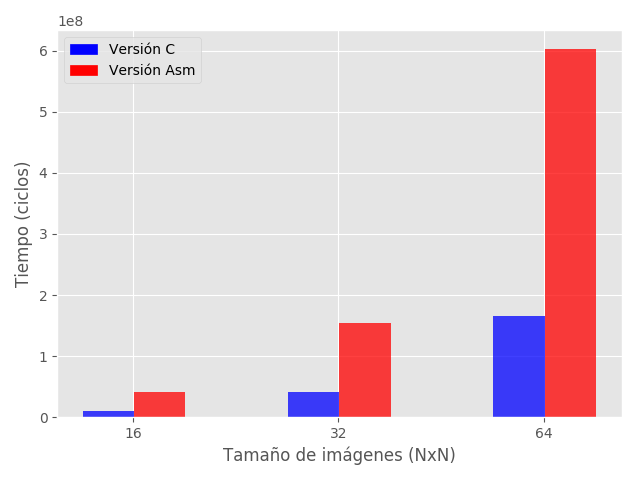
\includegraphics[width=0.8\textwidth]{imagenes/CvsAsm16-64.png}
\end{center}

\begin{center}
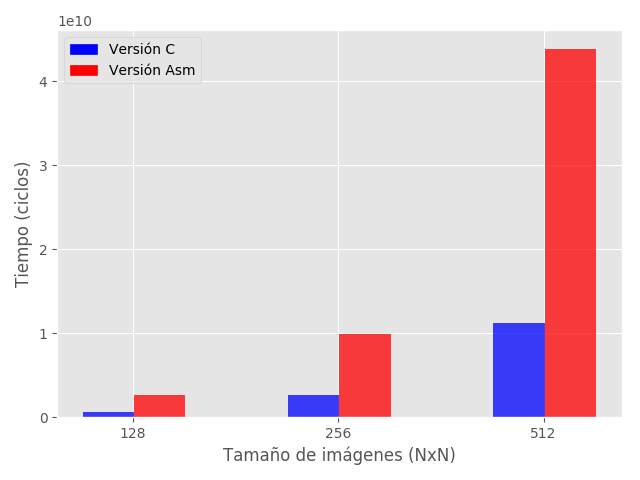
\includegraphics[width=0.8\textwidth]{imagenes/CvsAsm128-512.png}
\end{center}

En estos graficos se puede ver claramente que la implementacion en asm es mucho mas rapida y esta diferencia
crece aun más cuanto mas grande es la entrada. sin embargo en la proxima seccion se puede ver
en detalle como impacta en particular cada una de las funciones en el tiempo total.



\subsubsection{Una función en assembler a la vez}
Aqui se observa el tiempo de todo el programa de distintas formas, todo el codigo en C,
todo el codigo con solo una de las 3 funciones implementadas en asm y con dos casos para lin_solve
utilizando la version final (lin_solve) y la primera implementacion mas larga y compleja (lin_solve_largo)

\begin{center}
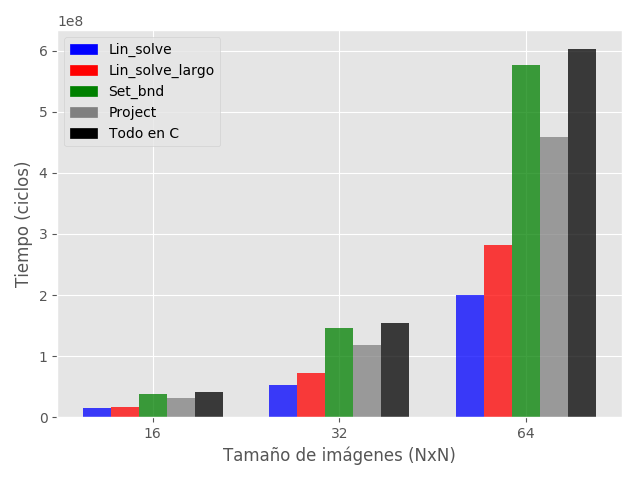
\includegraphics[width=0.8\textwidth]{imagenes/funciones16-64.png}
\end{center}

\begin{center}
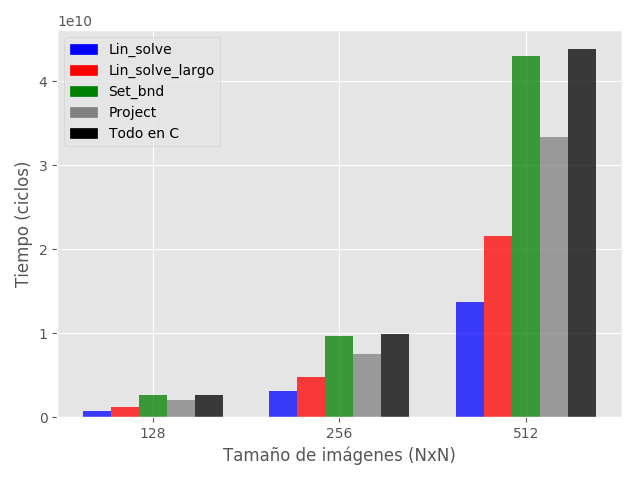
\includegraphics[width=0.8\textwidth]{imagenes/funciones128-512.png}
\end{center}

Analizando estos graficos, se puede ver que set_bnd, aunque presenta una mejoria, esta es infima
en comparacion a las otras funciones. Luego en el ranking viene project, la cual mejora el total del tiempo
pero aun asi ambas implementaciones de lin_solve representan la mayor parte de la mejoria de tiempo general.

Sindo lin_solve a su vez mejor que lin_solve_largo a pesar de que primero se creia lo contrario ya que
lin_solve_largo paraleliza mucho más y ejecuta menos ciclos. Sin embargo estos resultan más largos y aun más lentos en proporcion.

De aqui en adelante se trabaja con los tiempo medidos solo al principio y al final de la ejecucion de cada
funcion en particular en ambas implementaciones (C y asm) comparadas

\subsubsection{solver\_lin\_solve}
Se compara lin_solve final en asm contra lin_solve original en C.

\begin{center}
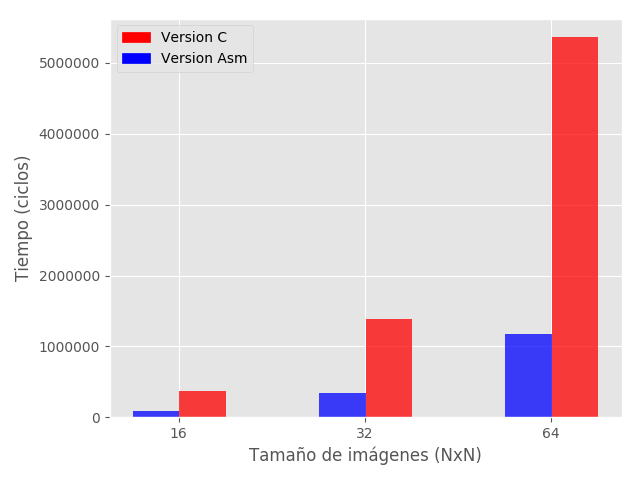
\includegraphics[width=0.8\textwidth]{imagenes/solver-lin-solve16-64.png}
\end{center}

\begin{center}
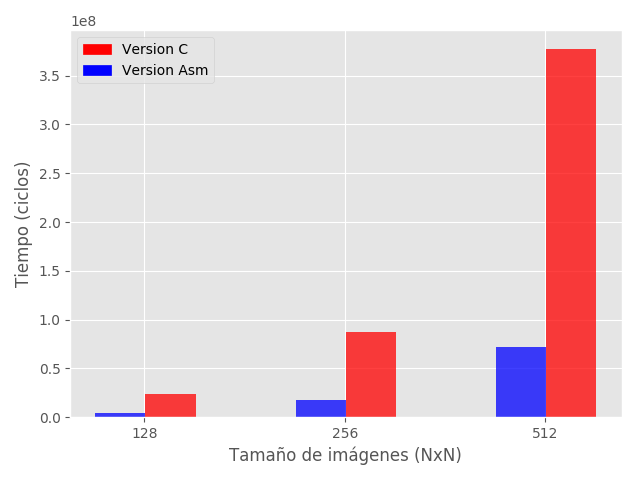
\includegraphics[width=0.8\textwidth]{imagenes/solver-lin-solve128-512.png}
\end{center}

Aqui se puede ver cuan abismal es la diferencia entre las versiones de lin_solve, cabe notar que nuestra
implementacion de lin_solve tiene un cambio en el orden de operaciones el cual facilita y acelera la ejecucion,
ademas de que el ciclo esta dividido en casos lo que reduce las comparaciones necesarias dentro del ciclo
y los simplifica sustancialmente.
Pero a pesar de ser matematicamente identica a la funcion original, el orden de operaciones afecta al
resultado final. Este tema sera visto con mejor detalle en la seccion diferencias.



\subsubsection{solver_set\_bnd}
Se compara set_bnd final en asm contra set_bnd original en C.

\begin{center}
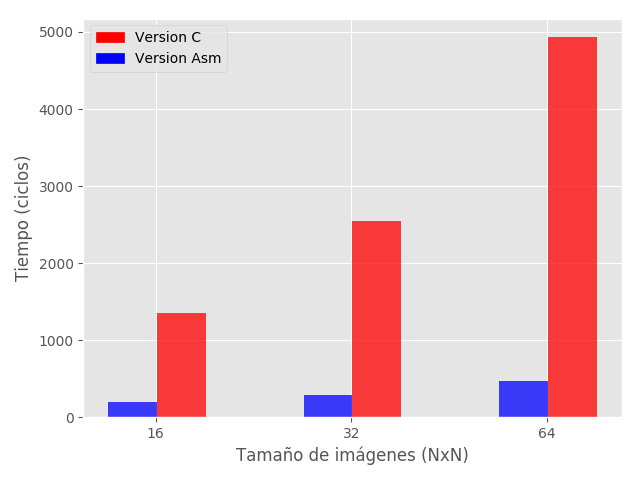
\includegraphics[width=0.8\textwidth]{imagenes/solver-set-bnd16-64.png}
\end{center}

\begin{center}
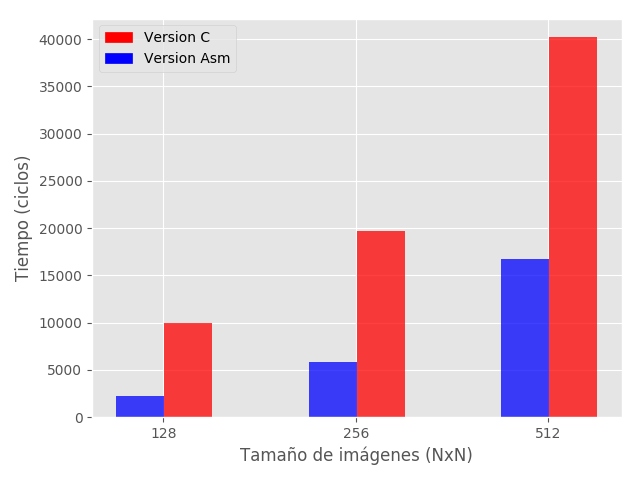
\includegraphics[width=0.8\textwidth]{imagenes/solver-set-bnd128-512.png}
\end{center}

Aqui se puede ver que set_bnd tambien presenta una buena mejora en asm respecto a C, pero notese que la escala
de tiempo es mucho más chica, lo cual muestra que la diferencia no significa mucho en cuanto al tiempo
total de la funcion, en otras palabras, la funcion set_bnd original ya ejecutaba pocos ciclos
en comparacion a las otras funciones y por eso la mejoria no es tan notable en lineas generales

\subsubsection{solver_project}
Se compara project final en asm contra project original en C.

\begin{center}
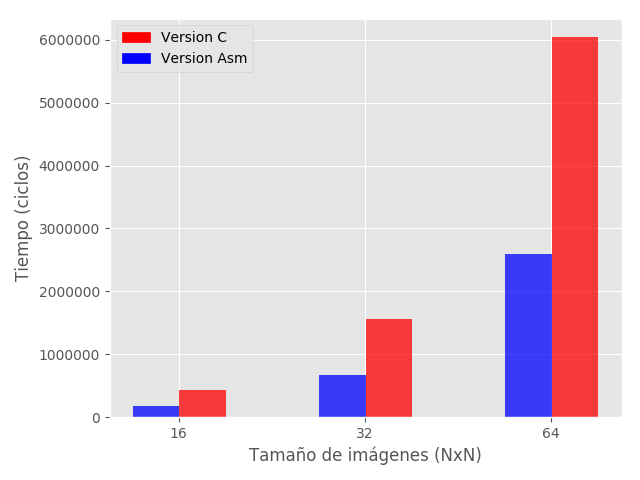
\includegraphics[width=0.8\textwidth]{imagenes/solver-project16-64.png}
\end{center}

\begin{center}
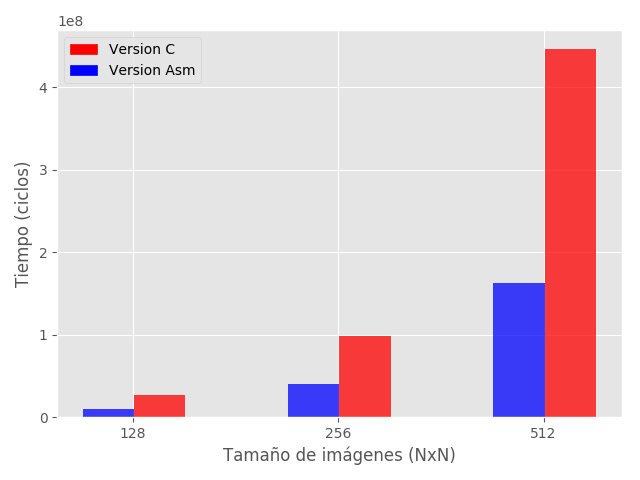
\includegraphics[width=0.8\textwidth]{imagenes/solver-project128-512.png}
\end{center}

Con project se puede ver que la implementacion en asm es muy buena en comparacion, pero la mejoria
es un poco menor que la que presenta lin_solve, y cuanto mas grande la entrada y al crecer exponencialmente
la diferencia entre C y asm,
mas se nota que lin_solve recude los tiempos en mayor medida, lo cual lleva a concluir
que lo visto en el primer grafico es acertado.





\subsection{Diferencias}

En esta seccion se observan las diferencias de las imagenes que corren los tests
en base a promedios y medianas.


Aqui se trabaja con todo el codigo en asm comparado al codigo original, notese que las
diferencias son en su totalidad causadas por la implementacion de lin_solve.


En primer lugar se decidio reescribir la funcion en C, modificando el orden de operacion
al realizar un factor comun, lo cual mantiene la logica matematica y facilita
la paralelizacion en asm y causa una mejoria temporal (como ya se vio en la seccion tiempo), pero introduce una diferencia
causada por el uso de floats, cuyos resultados si se ven afectados por el orden de operacion
sin importar la correctitud de la logica.
Entonces, ambos codigos en C (original y reescrito) ya presentaban una diferencia entre si.
Pero nuestra implementacion en asm, la cual se basa en la de C reescrita, no presenta ninguna diferencia
la misma, por lo cual decidimos mantener la implementacion como algo correcto.


No hay tablas para los tamaños de 16, 32 y 64 porque no hubo diferencias con las
versiones de la cátedra.

Promedio$_1$ es igual al promedio de todos los pixeles de la imagen

Promedio$_2$ es igual al promedio de solamente los píxeles que no son negros

Mediana$_1$ es igual a la mediana de todos los pixeles de la imagen

Mediana$_2$ es igual a la mediana de solamente los pixeles que no son negros

\begin{table}[H]
	\caption{Diferencias con la cátedra -- Tamaño $128\times128$} \label{tab:title}
	\begin{center}
		\begin{tabular}{| >{\centering\arraybackslash}m{0.9in} | >{\centering\arraybackslash}m{0.9in} | >{\centering\arraybackslash}m{0.9in} | >{\centering\arraybackslash}m{0.9in} |}
			\hline
			& \multicolumn{3}{c|}{\bf 128}\\
			\cline{2-4}
      & \bf Velocidad v & \bf Velocidad u & \bf Densidad \\\hline
      \bf Promedio$_1$ & 0.1113 & 0.9035 & 0.0015\\ \cline{2-4}
			\bf Promedio$_2$ & 1.0691 & 1.0096 & 1.0\\ \cline{2-4}
			\bf Mediana$_1$ & 0 & 1 & 0\\ \cline{2-4}
			\bf Mediana$_2$ & 1 & 1 & 1\\ \cline{2-4}
			\bf Cantidad & 1706 & 14662 & 25\\ \cline{2-4}
			\bf Maximo & 13 & 12 & 1\\ \cline{2-4}
			\hline
		\end{tabular}
	\end{center}
\end{table}

\begin{table}[H]
	\caption{Diferencias con la cátedra -- Tamaño $256\times256$} \label{tab:title}
	\begin{center}
		\begin{tabular}{| >{\centering\arraybackslash}m{0.9in} | >{\centering\arraybackslash}m{0.9in} | >{\centering\arraybackslash}m{0.9in} | >{\centering\arraybackslash}m{0.9in} |}
			\hline
			& \multicolumn{3}{c|}{\bf 256}\\
			\cline{2-4}
      & \bf Velocidad v & \bf Velocidad u & \bf Densidad \\\hline
      \bf Promedio$_1$ & 14.8418 & 0.0733 & 0.0740\\ \cline{2-4}
			\bf Promedio$_2$ & 14.8516 & 2.6657 & 9.9876\\ \cline{2-4}
			\bf Mediana$_1$ & 16 & 0 & 0\\ \cline{2-4}
			\bf Mediana$_2$ & 16 & 1 & 4\\ \cline{2-4}
			\bf Cantidad & 65493 & 1804 & 486\\ \cline{2-4}
			\bf Maximo & 105 & 39 & 129\\ \cline{2-4}
			\hline
		\end{tabular}
	\end{center}
\end{table}

\begin{table}[H]
	\caption{Diferencias con la cátedra -- Tamaño $512\times512$} \label{tab:title}
	\begin{center}
		\begin{tabular}{| >{\centering\arraybackslash}m{0.9in} | >{\centering\arraybackslash}m{0.9in} | >{\centering\arraybackslash}m{0.9in} | >{\centering\arraybackslash}m{0.9in} |}
			\hline
			& \multicolumn{3}{c|}{\bf 512}\\
			\cline{2-4}
      & \bf Velocidad v & \bf Velocidad u & \bf Densidad \\\hline
      \bf Promedio$_1$ & 1.5447 & 1.8360 & 0.1312\\ \cline{2-4}
			\bf Promedio$_2$ & 1.5721 & 1.8495 & 3.6362\\ \cline{2-4}
			\bf Mediana$_1$ & 1 & 2 & 0\\ \cline{2-4}
			\bf Mediana$_2$ & 1 & 2 & 2\\ \cline{2-4}
			\bf Cantidad & 257571 & 260225 & 9463\\ \cline{2-4}
			\bf Maximo & 61 & 30 & 48\\ \cline{2-4}
			\hline
		\end{tabular}
	\end{center}
\end{table}

De estas tablas se puede ver que, logicamente, cuanto mas grande la imagen mas pixeles distintos,
pero tambien se puede ver que estos pixeles distintos no alcanzan valores muy grandes, y las medianas
y los promedios se mantienen siempre muy bajo, lo cual marca que a pesar de haber diferencias, estas no son
abismales.


Pero extrañamente la matrix de 256 x 256 se comporta mucho peor que la de 512 x 512 más grande, esta ultima
presenta más pixeles con diferencias, pero la primera tiene diferencias mucho más grandes de hasta un poco sobre la mitad
del rango de color. Realmente no pudimos explicar este comportamiento.


Tambien se ve que la matriz densidad es por mucho la menos afectada en cantidad de pixeles distintos y en
diferencias en general, asumimos que esto se da porque la matriz de densidad pasa una sola vez por lin_solve por ciclo,
cuando las matrices de velocidad pasan almenos dos veces por lin_solve en cada ciclo.
